%\title{\LARGE \bf A Shared Control Method for Online Human-in-the-Loop Robot Learning Based on Locally Weighted Regression}

%\author{Luka Peternel$^{\text{a},}$$^{\text{c}}$, Erhan Oztop$^{\text{b}}$ and Jan Babi\v{c}$^{\text{c}}$% <-this % stops a space
%\thanks{$^{\text{a}}$HRI$^2$ Lab, Dept. of Advanced Robotics, Istituto Italiano di Tecnologia, Genoa, Italy, Email: luka.peternel@iit.it}
%\thanks{$^{\text{b}}$Robotics Laboratory, \"{O}zye\u{g}in University, Istanbul, Turkey}
%\thanks{$^{\text{c}}$Dept. of Automation Biocybernetics and Robotics, Jo\v{z}ef Stefan Institute, Ljubljana, Slovenia}
%\thanks{This work was supported by the EC Framework Programme 7 through the CoDyCo project (\#600716) and the Converge project (\#321700).}}


\section{Introduction}
\label{sec:introduction}
Robot learning can be a good alternative to time-consuming classical manual programming that requires experts and expert time. One such example is reinforcement learning where the robot autonomously learns the task through the trial-and-error principle \cite{Kober2012}. Another example is learning-by-demonstration where the human directly demonstrates the robot how to perform a given task \cite{Hersch2008,Evrard2009,Ude2010,Amor2009,Nguyen2009,Peternel2013b,Gams2009,Peternel2014}.

Robot learning-by-demonstration can be generally divided into offline and online type of learning \cite{Nguyen2011}. In offline learning the training data is acquired in the demonstration stage, and subsequently the training data is used in combination with a machine-learning method to form a robotic skill, which can be later used by the robot in the autonomous stage \cite{Hersch2008,Evrard2009,Ude2010,Ewerton2015}. The advantage of this approach is that the demonstrator can select the best data or adjust it in order to achieve the best learning performance. The key drawback of pure offline learning in the teaching-by-demonstration framework is that the human demonstrator does not have any feedback about the robot learning {\it during} the demonstration stage. The actual performance of the obtained robotic skill by using the data collected during demonstration can only be observed later in the autonomous stage. If the autonomous performance is unsatisfactory then the whole procedure has to be repeated.

Above-mentioned drawback can partially be addressed by multiple demonstrations to obtain some variety that can benefit the obtained robotic skill during the autonomous stage \cite{Ewerton2015}. Alternatively, the skill obtained during the demonstration stage can be corrected by the human in the autonomous stage through social interaction \cite{Nicolescu2003,Lockerd2004,Argall2007}. However, this method requires relatively high level of robot intelligence to recognise the human advice and devise a strategy to correct its performance on sensorimotor level. If the task is complex, the correction procedure may be time-consuming and in some cases unsuccessful. Therefore, another direct sensorimotor-level demonstration from the human could be faster and more efficient.

Contrary to offline learning, in online learning the robotic skill is formed gradually already during the demonstration stage \cite{Nguyen2011}. One of the advantages of this is that the transition between demonstration stage and autonomous stage can be direct and automatic \cite{Peternel2013b,Gams2009,Peternel2014}. Importantly, online learning also allows the demonstrator to get useful feedback about the performance of the robotic skill being constructed during the demonstration \cite{Lee2011,Peternel2013b,Peternel2016}. In this case, the correction of the obtained skill can be performed online and directly on sensorimotor level \cite{Lee2011,Peternel2016}, and it can therefore be faster and less complicated from the user perspective.

In \cite{Lee2011}, the authors proposed a kinaesthetic teaching method that allows the demonstrator to incrementally improve the the currently leant robotic skill. The skill refinement is done by physical interaction at low robot stiffness. However, in kinaesthetic teaching the immersion of demonstrator is limited, especially with regards to tactile sensing. In addition, simultaneous online demonstration of impedance \cite{Peternel2014,Peternel2015} can be difficult. These drawbacks can be addressed by teleoperation-based teaching \cite{Evrard2009,Peternel2013b,Peternel2014}. However, in this approach the control commands for the robotic mechanism are simultaneously generated by both the human demonstrator and by the robot control policy (represented as a non-linear function approximator) being learnt \cite{Peternel2013b}. Therefore, a mechanism that arbitrates the control responsibility over the target robotic platform is required to enable the co-adaptation between the involved agents.

\section{Related Work}
\label{sec:related}
While shared control is a well-studied subject in teleoperation \cite{Niemeyer2008,Dragan2013} and assistive robotics \cite{Omalley2006,Dragan2013,Jain2015,Peternel2016}, there are only a few studies that investigated shared control on a sensorimotor level in the teleoperation-based human-in-the-loop robot teaching. Study in \cite{Peternel2013b} proposed a method to share the control between the demonstrator and robotic skill in an online robot learning scenario based on Locally Weighted Regression (LWR) \cite{Schaal1998,Vijayakumar2005} machine learning. The control-sharing algorithm defined the amount of control responsibility of each agent as a ratio based on the prediction error, i.e. the average error between the human generated motor output and LWR output. The reasoning was that when the machine-learning algorithm learns to replicate human generated motor commands reliably then the control could be shifted to the machine control. This works very well when the demonstrator quickly becomes an expert in performing the task at hand \cite{Peternel2013b}.

Study in \cite{Zamani2015} developed a variant of the approach proposed in \cite{Peternel2013b} by designing a new strategy for determining the control arbitration. Instead of using prediction error to adjust the control sharing, they used a local success measure of the task execution, which does not directly depend on the prediction error of the machine-learning module. This is beneficial for tasks where the human demonstrator needs time to adapt to task to perform well; because this does not allow the machine to learn a bad policy by simply becoming a very good imitator of a bad demonstrator. The local success measure is somewhat analogous to introducing virtual rewards to speed-up learning in the reinforcement-learning framework. The disadvantage of this approach is the additional complexity and task dependency. For a useful local success measure the task must be well defined and should naturally facilitate local success definition, by for example, allowing state space decomposition into subtasks. Naturally, some tasks do not meet these conditions, and for those that meet, the one-time expert effort might be non-negligible.

The two approaches in \cite{Peternel2013b} and \cite{Zamani2015} described above both advocate a control sharing mechanism between the agents. This means the performance of the robot during demonstration is a mixture of human and machine control. Here we have two potentials difficulties for the human demonstrator. (1) The credit assignment problem: it may be difficult to determine whether the current unsatisfactory performance of the robot is due to the control commands from the demonstrator or the machine-learning module. (2) The non-stationarity problem: how the robot responds to the human control commands that change with time and in a complex way; this must be an initial burden for human demonstrators \cite{Zamani2015}.

In this paper we propose and investigate a new shared-control approach for teleoperation-based human-in-the-loop online robot teaching that addresses the two difficulties indicated above. Contrary to \cite{Peternel2013b} and \cite{Zamani2015}, we adopt a binary control responsibility scheme where the control is either fully delegated to the demonstrator or to the machine-learning module. This allows the demonstrator to clearly know who is responsible for the ongoing task execution performance. In addition, the approach retains the simplicity from the user perspective \cite{Peternel2013b} as it does not require the task and reward function to be defined in advance. In \cite{Peternel2013b} the control is delegated gradually based on the average error between the human and robotic skill performance over the entire state space up until the current observation time. The disadvantage of this is that human cannot efficiently inspect the robotic skill performance locally in a specific state region. Contrary to that, in the proposed method the control is delegated based on the existence of local models in specific state regions. This gives the demonstrator an option to freely inspect the performance of the robotic skill in any specific state region (and if necessary to correct it).

\section{Methods}
In the proposed approach, the control sharing is based on a mechanism that exploits the machine-learning method (LWR) adopted \cite{Schaal1998,Vijayakumar2005}. LWR builds a non-linear model by creating local linear models over non-linear basis functions that have local span (i.e. receptive fields) over the states and are incrementally generated during task demonstration. The existence or nonexistence of local models (in the LWR module) in a given state region is used to arbitrate control: when the robot finds itself in a state region where no local models exist the control is given to the human demonstrator so that new models can be learnt. If the current state of the robot is within the proximity of a local model (i.e. it activates the receptive field of some model) then the control is given to the machine-learning module. This allows the human to examine the performance of the current robotic skill during the demonstration stage. If the performance is unsatisfactory the teaching can be repeated and models can be updated/replaced in the given state region.
\begin{figure}[!t]
  \centering
  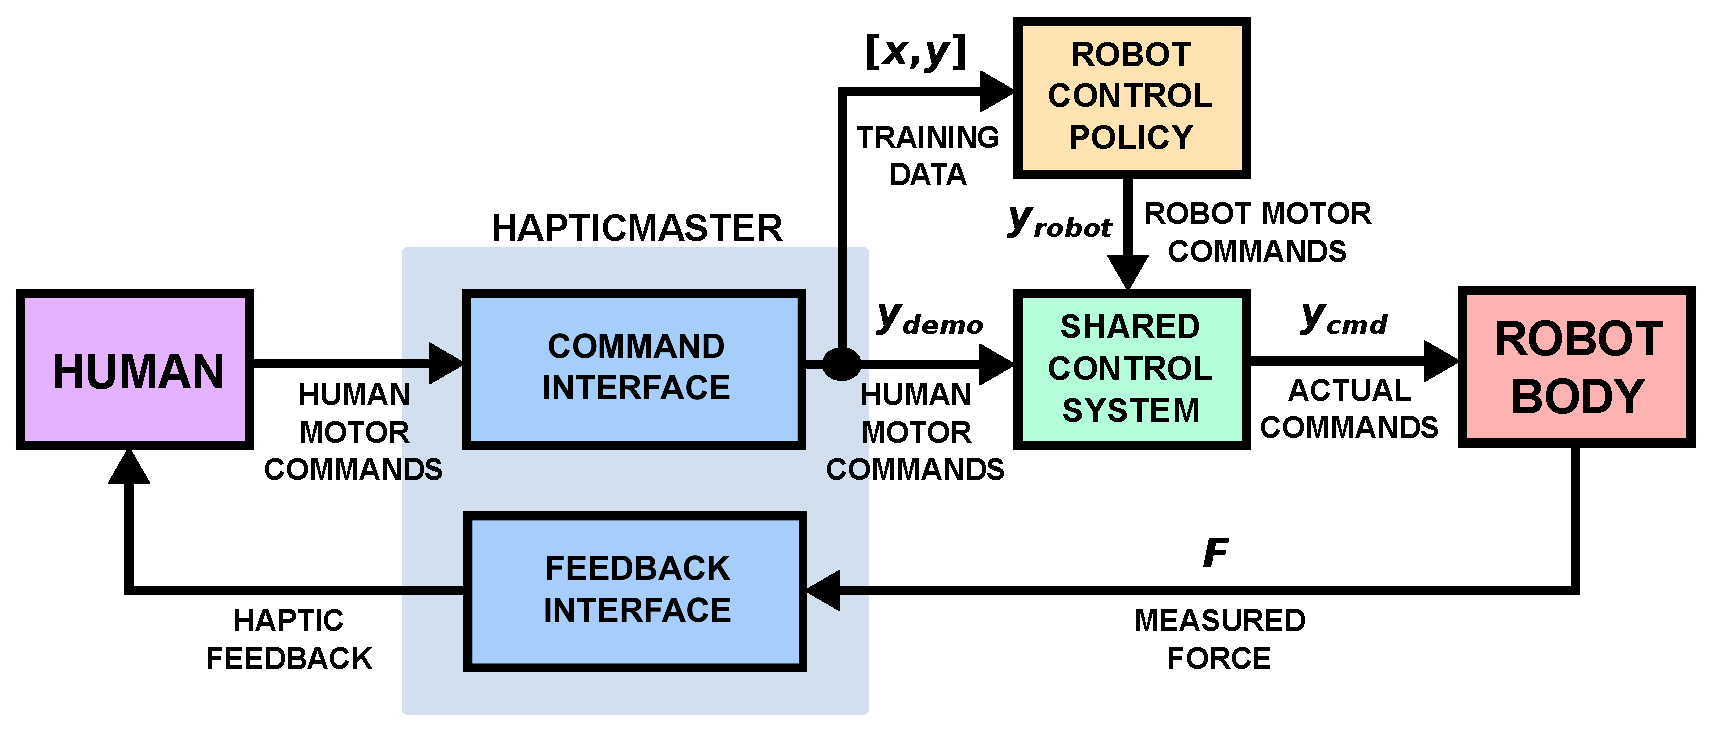
\includegraphics[width=0.70\textwidth]{Luka/scheme.eps}
  \caption{The proposed human-in-the-loop teaching approach with shared control between the actions of demonstrator ($y_{demo}$) and robotic skill ($y_{robot}$). HapticMaster robot serves as an interface between the demonstrator and the controlled robotic manipulator.}
  \label{fig:scheme}
  \vspace{-4 mm}
\end{figure}

To demonstrate and validate the concept of the proposed method we performed experiments on a Moog HapticMaster (HM) robot. The task of the robotic manipulator was to produce a reference force between its end-effector and unknown objects in the environment. The surfaces of the objects had different stiffness. The task of the human demonstrator was to teach the robotic manipulator how to adjust the commanded (reference) position in order to maintain the predefined force over the entire operational space (plane).

The human demonstrator was included into the robot control loop by a human-robot interface as shown in Fig. \ref{fig:scheme}. The HM robot served as the necessary control interface for the virtual robotic manipulator that needs to be manoeuvred to achieve a constant vertical force feedback over an environment that has non-homogenous stiffness. While operating the robot trough this teleoperation setup, the human demonstrator could easily gain the skill to perform the task through the robot. After an initial practice session, the skill demonstration stage was started where the human demonstrator taught the robot how to perform the desired task. Simultaneously, the robot acquired the skill incrementally in real-time as detailed below. The proposed control arbitration mechanism delegated the control to the demonstrator or to the so-far-built robot control policy (robotic skill). The control policy learning was inhibited for the state regions where sufficient level of learning was already attained, and the robot was commanded using this learnt policy. In contrast, when the robot entered a state region where sufficient learning did not take place, the control was granted to the demonstrator and the learning resumed.


\subsection{Locally Weighted Regression}
The LWR method\footnote{LWR is used here for generality. Locally Weight Projection Regression\cite{Vijayakumar2005} can be used in our method instead to cope with higher dimensionality.} is an incremental (online) function approximator that can be used to represent {\it output} as a function of {\it input} given a set of [input, output] pairs, i.e. the training data points. To do this, it forms local expert models that are responsible for particular input regions. Each local expert is a linear model and is assumed to represent its responsibility area. The output prediction $\hat{\bm{y}}(\bm{x})$, for some new input $\bm{x}$, is given by the sum of contributions of all local models \cite{Schaal1998}
\begin{equation}
\hat{\bm{y}}(\bm{x}) = \frac{\sum\limits_{i=1}^N w_{i}\bm{y}_{i}^{model}}{\sum\limits_{i=1}^N w_{i}},
\label{eq:lwr1}
\end{equation}
where $\bm{y}_{i}^{model}$ is the prediction of the $i^{th}$ local model, and $w_{i}$ its weight. Weights determine the contribution of each local model in the final prediction, $\hat{\bm{y}}$ given input $\bm{x}$. Weights are computed by the activation of models' receptive fields defined by Gaussian kernel functions \cite{Schaal1998}
\begin{equation}
w_{i} = \exp\big(-\frac{1}{2}(\bm{x}-\bm{c}_{i})^{T}\bm{D}_{i}(\bm{x}-\bm{c}_{i})\big),
\label{eq:lwr2}
\end{equation}
where $\bm{D}_{i}$ is positive definite matrix that contains information about the size of receptive field. Parameter $\bm{c}_{i}$ represents the centre of the receptive field and its local model. By observing (\ref{eq:lwr2}) one can notice that the influence (weight) of a local model $\bm{y}_{i}^{model}$ decreases with the distance of input $\bm{x}$ from the centre $\bm{c}_{i}$ of that model.

Local linear models are defined as \cite{Schaal1998}
\begin{align}
	\bm{y}_{i}^{model} &= (\bm{x} - \bm{c}_i)^{T} \bm{m}_i + m_{0,i} = \tilde{\bm{x}}_{i}^{T}\bm{M}_{i},\label{eq:lwr3}\\
	\tilde{\bm{x}} &= [(\bm{x}-\bm{c}_{i})^{T},1]^{T},\label{eq:lwr4}
\end{align}
where $\bm{y}_{i}^{model}$ is the i-th model prediction given the input $\bm{x}$, while $\bm{c}_{i}$ is the centre of the $i^{th}$ model. Vector $\bm{M}_{i}$ contains the parameters that describes the local model and $\tilde{\bm{x}}$ is the distance from the centre of the model.

The learning process needs to determine model parameters $\bm{M}_{i}$, centre parameters $\bm{c}_{i}$ and distance metrics $\bm{D}_{i}$ that determines the size of the model's receptive field. The learning is done incrementally while the training data are fed to the learning system. Each training data point $[\bm{x},\bm{y}]$ updates the existing models via  recursive least-square method \cite{Schaal1998}
\begin{align}
\bm{M}(k+1) &= \bm{M}(k) + w \bm{P}(k+1) \tilde{\bm{x}} \bm{e}_{lwr}^{T},\label{eq:lwr5} \\
\bm{e}_{lwr} &= (\bm{y}-\bm{M}(k)^{T}\tilde{\bm{x}}),\label{eq:lwr6} \\
\bm{P}(k+1) &= \frac{1}{\lambda}\left(\bm{P}(k)-\frac{\bm{P}(k)\tilde{\bm{x}}\tilde{\bm{x}}^{T}\bm{P}(k)}{\frac{\lambda}{w}+\tilde{\bm{x}}^{T}\bm{P}(k)\tilde{\bm{x}}}\right) ,\label{eq:lwr7}
\end{align}
where $\lambda$ forgetting factor that allows the system to gradually forget the previously demonstrated training data points.

Adjustment of model's receptive field size is performed by a modified leave-one-out cross-validation method \cite{Schaal1998}. As new training data points are used for the LWR update, new local models are created - and in same cases removed, to facilitate a parsimonious distribution of the local models across the input space. A new model is created when a training point $[\bm{x},\bm{y}]$ does not active any of the receptive fields more than a threshold $w_{gen}$ \cite{Schaal1998}, and the centre of the newly created model is set to the position of the new training point ($\bm{c}=\bm{x}$). When a training point activates two receptive fields simultaneously for more than a predetermined threshold $w_{prune}$, then the model with the larger covariance matrix is removed \cite{Schaal1998}. This prevents unnecessary overlap of the models that would lead to computational inefficiency.

\subsection{Shared-Control Approach}
We delegated the control over the robotic mechanism between the human and robotic skill by the following expression \cite{Peternel2013b} (see also Fig. \ref{fig:scheme})
\begin{equation}
\bm{y}_{cmd} = C \cdot \bm{y}_{demo} + (1-C) \cdot \bm{y}_{robot} ,
\label{eq:delegation}
\end{equation}
where $\bm{y}_{cmd}$ is a vector of commands sent to the robotic mechanism, $\bm{y}_{demo}$ is a vector of commands given by the human demonstrator, $\bm{y}_{robot}$ is a vector of commands produced by the current robotic skill and $C \in [0,1]$ is a weight factor that determines the influence of each agent. Pure human control is achieved when $C = 1$, and pure machine control is achieved when $C = 0$.

In our method, we used the information about the current state of the local models in LWR to determine the value of the factor $C$. When the demonstrator is performing the task in a state (i.e. position on the plane) where a feasible local model exists the task execution is purely based on the current robot control policy that is represented by (\ref{eq:lwr1}), and learning is inhibited. If no local model is present in the current robot state then the control of the task execution is given to the demonstrator, and teaching is resumed. To determine the proximity to the local model we used the activation $w_{max}$ of the model that provides the maximum activation for the current position of the input vector $\bm{x}$. We defined factor $C$ as
\begin{equation}
C = \begin{cases} 1 & \text{if } w_{max} < (w_{th} - \frac{d}{2})
\\ \frac{ 1 + \cos \big(\pi \frac{w_{max} - (w_{th} - \frac{d}{2}) }{d}\big)}{2}  & \text{if } (w_{th} - \frac{d}{2}) \leq w_{max} \leq (w_{th} + \frac{d}{2}),
\\ 0 & \text{if } w_{max} > (w_{th} + \frac{d}{2}) \end{cases}
\label{eq:factor}
\end{equation}
where $w_{max}$ is the strongest activation of the model receptive fields \cite{Schaal1998} and $w_{th}$ is an activation threshold that we introduced to determine the model-proximity based shared control. Although, the main regime for $C$ is binary, we used a cosine based function to prevent sudden jumps in net control output and to facilitate smooth transitions between human control and machine control modes of operation. Here the parameter $d$ defines the width of switching function, and thus should be assigned a small value to obtain the desired binary regime.

During the demonstration stage the training data is collected and accumulated for a predefined sample length before it is fed to the LWR-based learning system. Instead of feeding the data to LWR in the order it is received, a random order can improve the learning at lower $\lambda$. Data accumulation takes place only when the human demonstrator has control over the robot (i.e. control factor $C = 1$). When appropriate LWR models exist in a given state region, the robot behaves autonomously by following the control policy dictated by the active LWR models (i.e. control factor $C = 0$). The data accumulation is paused in this case, until when the user gains full control again. The described approach can be described as
\begin{equation}
\bm{A}_{new} = \begin{cases} \bm{A} & \quad \text{if } C \neq 1
\\ [\thinspace \bm{A}; \thinspace [\bm{x}, \thinspace \bm{y}]\thinspace ] & \quad \text{if } C = 1 \text{ \& } \text{length}(\bm{A}) < N_{acc},
\\ [\thinspace] & \quad \text{if } \text{length}(\bm{A}) = N_{acc} \\ \end{cases}
\label{eq:accumulate}
\end{equation}
\begin{equation}
\bm{A}_{in} = \bm{A}\big(\text{randperm}(N_{acc}),\thinspace :\big),
\label{eq:shuffle}
\end{equation}
where $\bm{A}$ is the matrix (accumulation buffer) where the training data is accumulated, and the notation $\bm{A}_{new}$ indicates that $\bm{A}$ is updated at each iteration. $N_{acc}$ is the predefined accumulation sample length that determines the amount of data that is fed to LWR in each update epoch. As mentioned above, a shuffling is applied before the data is fed to LWR, so instead of $\bm{A}$, $\bm{A}_{in}$, the random shuffled version of it is used. If we want to accumulate a large data set before each update then it is reasonable to reduce its size by also applying down-sampling before the shuffling.

The final transition from the demonstration stage to the fully autonomous stage (human demonstrator disconnected from the robot control loop) can be either done automatically or manually. The automatic switch can be realised based on the threshold percentage of the given task space being covered by the local models.


\section{Experimental Setup}
In the experiments we used HM robot as an interface between the human demonstrator and the robotic manipulator (see Fig. \ref{fig:setup}). Please refer to the supplementary multimedia file for a video of the setup/experiment. HM has a robotic arm with 3 active degrees of freedom that can render a haptic environment at the end-effector where the human holds and moves it. At the same time HM provides the measured position of the end-effector that can be used to command the position of the teleoperated robotic manipulator. The physical aspects of the robotic manipulator and the environment were simulated in MATLAB/Simulink, while the visual aspects were simulated by the OpenGL Utility Toolkit (GLUT) (see Fig. \ref{fig:surface}). The robot was positioned in front of the demonstrator who sat on a chair. We mounted a monitor in front of the demonstrator where we displayed the virtual environment and feedback related to the task execution. The machine-learning algorithm was based on the toolbox provided by \cite{Klanke2008}. The learning and shared-control algorithm operated at 100 Hz.
\begin{figure}[!t]
  \centering
  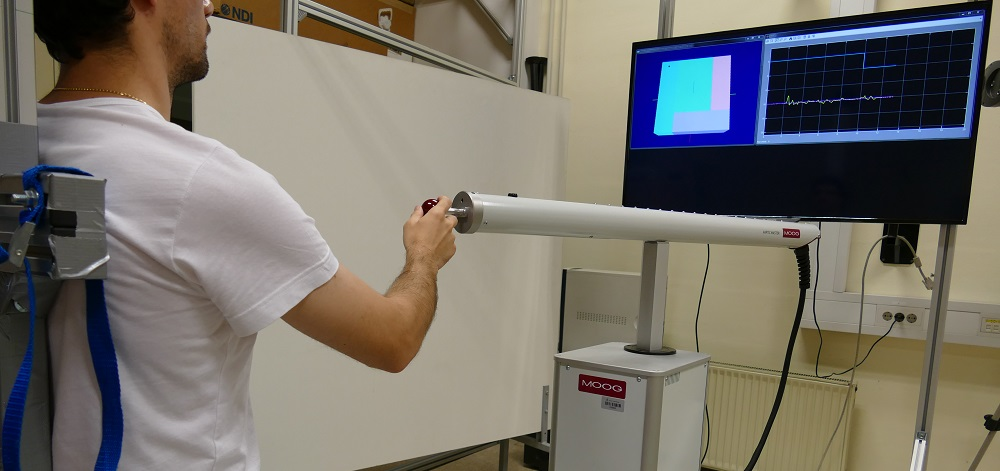
\includegraphics[width=0.6\textwidth]{Luka/setup.jpg}
  \caption{Robot manipulator control interface consisting of HapticMaster robot and monitor for providing human with visual feedback.}
  \label{fig:setup}
  \vspace{-2 mm}
\end{figure}
\begin{figure}[!t]
  \centering
  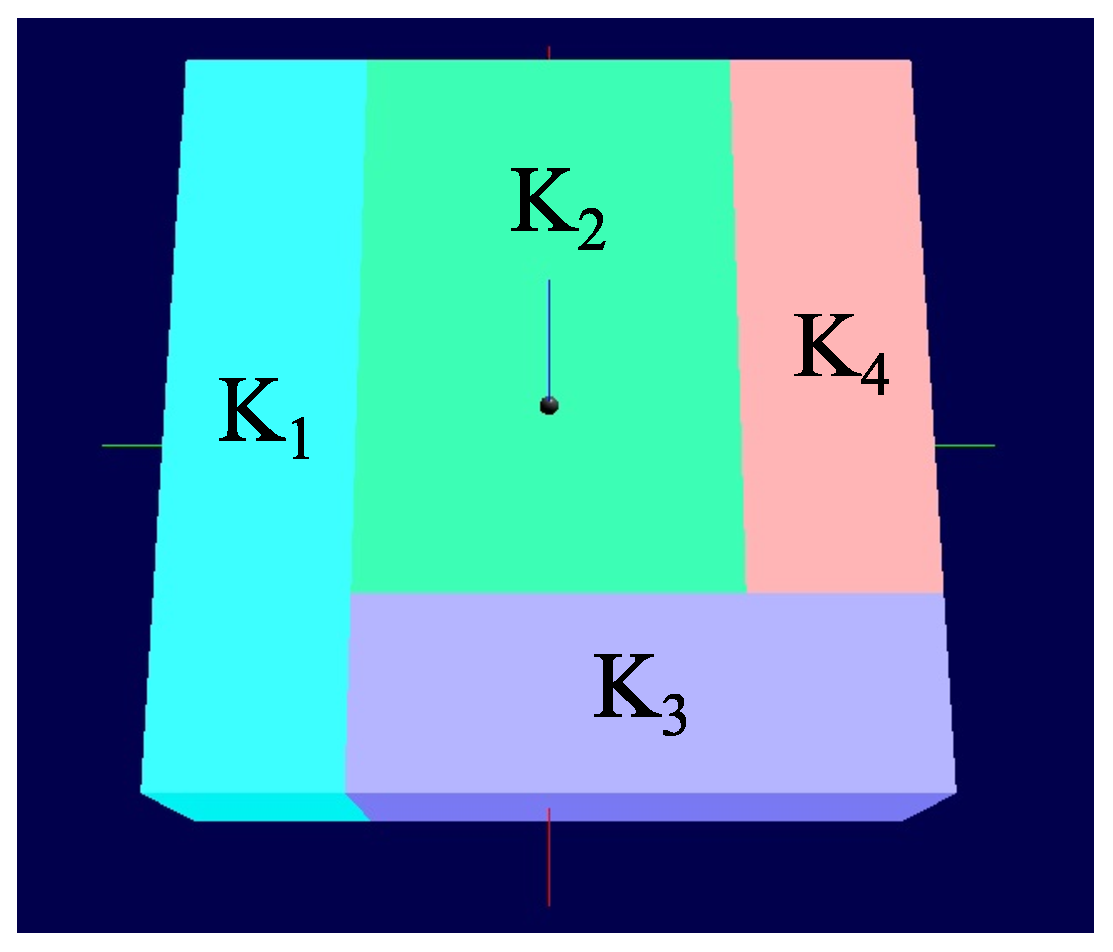
\includegraphics[width=0.4\textwidth]{Luka/env.eps}
  \caption{Virtual environment. The colours represent different objects on the surface. Each object has a different stiffness ($K_1$, $K_2$, $K_3$ and $K_4$). The robotic manipulator's actual end-effector position is displayed by the black ball in the centre.}
  \label{fig:surface}
  \vspace{-4 mm}
\end{figure}

The HM robot operated in two modes. The first mode was admittance control where the measured interaction force between the HM end-effector and human hand produced the desired motion. This mode was used in case when the demonstrator had the control over the virtual robotic manipulator ($C=1$). The actual position of the HM end-effector (human demonstrator's arm end-effector) was used as the commanded (reference) position for the virtual robotic manipulator. The actual position of the manipulator was dependant on the surface in the virtual environment. We assisted the demonstrator in precise maintaining the desired commanded position in z-axis by a virtual spring-damper system. The second mode was position control using a proportional controller realised by a virtual spring between the reference and actual HM end-effector position in z-axis. This mode was used in case when the robotic skill had the control over the virtual robotic manipulator ($C=0$).

One experienced human demonstrator participated in the experiments. The task of the robotic manipulator was to produce a reference interaction force on the unknown objects in the environment. The interaction force had to be produced perpendicularly to objects (in z-axis). Each object had different stiffness properties. To maintain the desired force the demonstrator had to adjust the commanded (reference) end-effector position in z-axis of the robotic manipulator based on the position in x-y plane. Please note that variables $x$ and $y$ now correspond to the position of robotic manipulator's end-effector. The following equation describes the necessary force control policy
\begin{equation}
	F_{z} = K(x,y) \big(z_r-z_a\big),\label{en:robotimp}
\end{equation}
where $F_{z}$ is the interaction force acting between the manipulator and the environment in z-axis, $K(x,y)$ is the stiffness of the object in z-axis, $z_a$ is actual and $z_r$ is reference position of the manipulator's end-effector in z-axis. The stiffness $K(x,y)$ depends on the object (i.e. on the position in x-y plane). Actual position $z_a$ depends on the environment too as the object blocks it from reaching the reference position inside the object. The higher the desired force is at a given stiffness of the object the larger the difference between commanded and actual position must be (i.e. reference must be deeper inside the object). For producing the same force, the difference between the commanded and actual position must be lower for objects with higher stiffness and vice-versa.

\begin{figure*}[!ht]
  \centering
  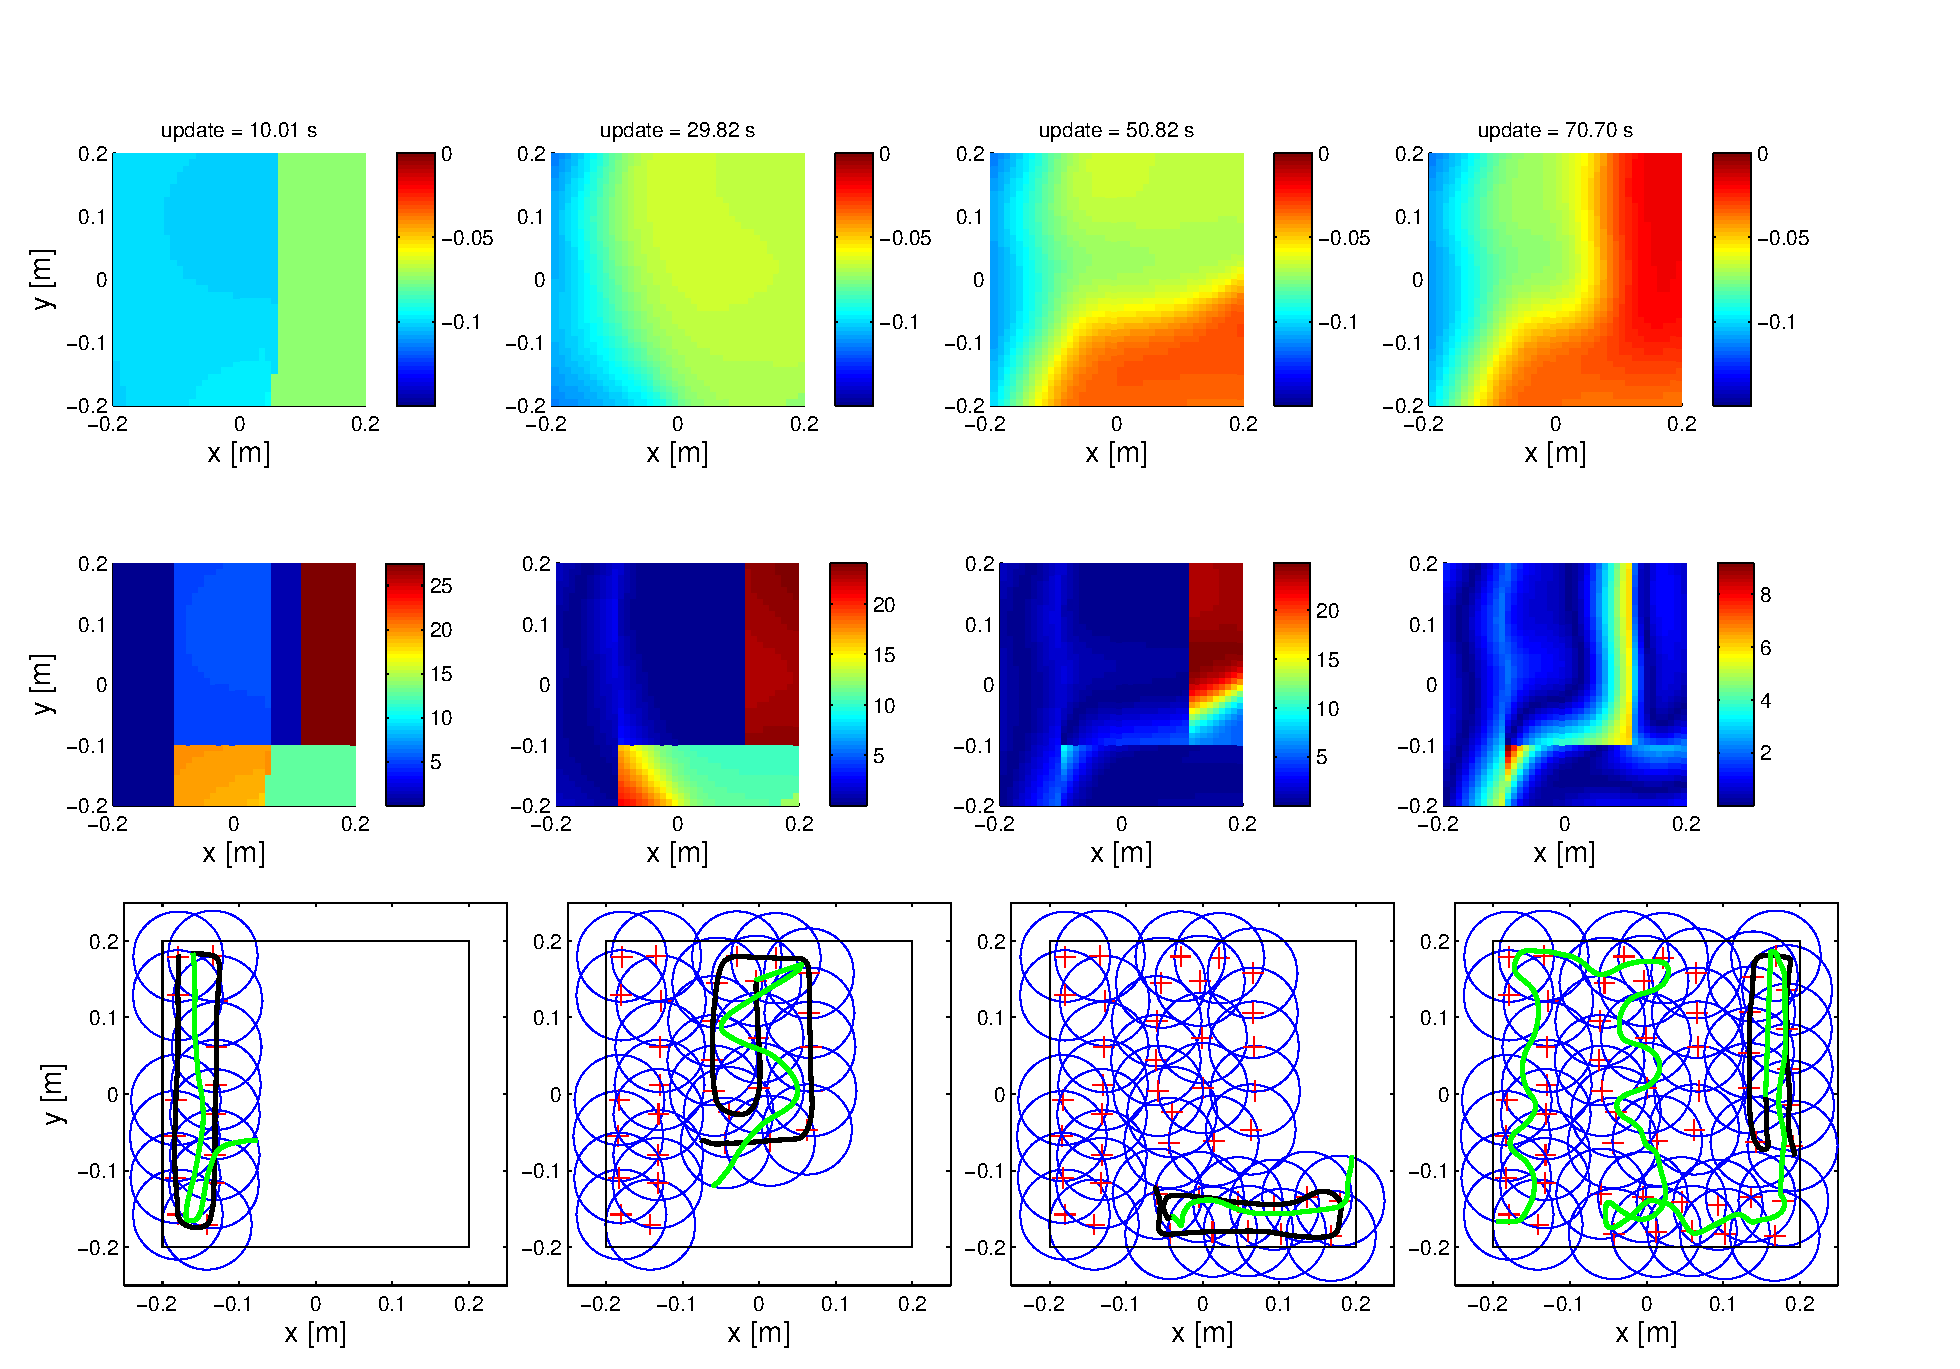
\includegraphics[width=0.85\textwidth]{Luka/results1.eps}
  \caption{Results of the experiments - learning. The top row graphs show prediction of robotic manipulator's commanded (reference) position displacement from the actual position in z-axis. The middle row graphs show the error of predicted interaction force in z-axis. The bottom row graphs show the motion trajectory in x-y plane (thick black line corresponds to $C=1$, thick green line corresponds to $C=0$) and distribution of local models (red crosses are centres and blue ellipses are activation ranges of $w_{th}$). Each column represents the state of robotic skill after training data update (update time stamps are on the top).}
  \label{fig:models}
  %\vspace{-4 mm}
\end{figure*}

We constructed a $0.4$ by $0.4$ meter surface from four different objects. The configuration of surface is shown in Fig. \ref{fig:surface}. Each object had a different stiffness: $k_1=100$ N/m, $k_2=150$ N/m, $k_3=300$ N/m and $k_4=500$ N/m. The goal was to teach the robotic manipulator how to produce a reference force $F_z=10$ N (LWR output) perpendicularly to the surface regardless of the position on the x-y plane (LWR input). The human demonstrator had to move the manipulator's position on x-y plane across various parts of the surface and the commanded position in z-axis had to be adjusted so that the reference force was maintained according to (\ref{en:robotimp}). While doing this, the learning system gradually acquired the skill how to produce the task autonomously. If the models existed in the given state region of x-y plane the shared-control system delegated the control responsibility over the manipulator to the robotic skill. Otherwise, the demonstrator had the control in order to continue the teaching process.

We determined parameters for the LWR-based learning system experimentally. The parameter related to the size of the model was set to $\bm{D} = \begin{bmatrix} 400 & 0 \\[0.3em] 0 & 400\end{bmatrix}$. The values of diagonal elements correspond to each input. Since in our case the inputs are the same physical quantity (position in x and y-axis), we set both diagonal elements to equal value. In case the inputs are different physical quantities then the values should be appropriately set for each input separately. Parameters related to the generation and removal of the models were set to $w_{gen}=0.8$, $w_{prune}=0.9$. For these proof-of-concept experiments selected $\lambda=1$ since we did not want to forget the old training data. If forgetting of older data is preferred then $\lambda < 1$ should be used.
\begin{figure*}[!ht]
  \centering
  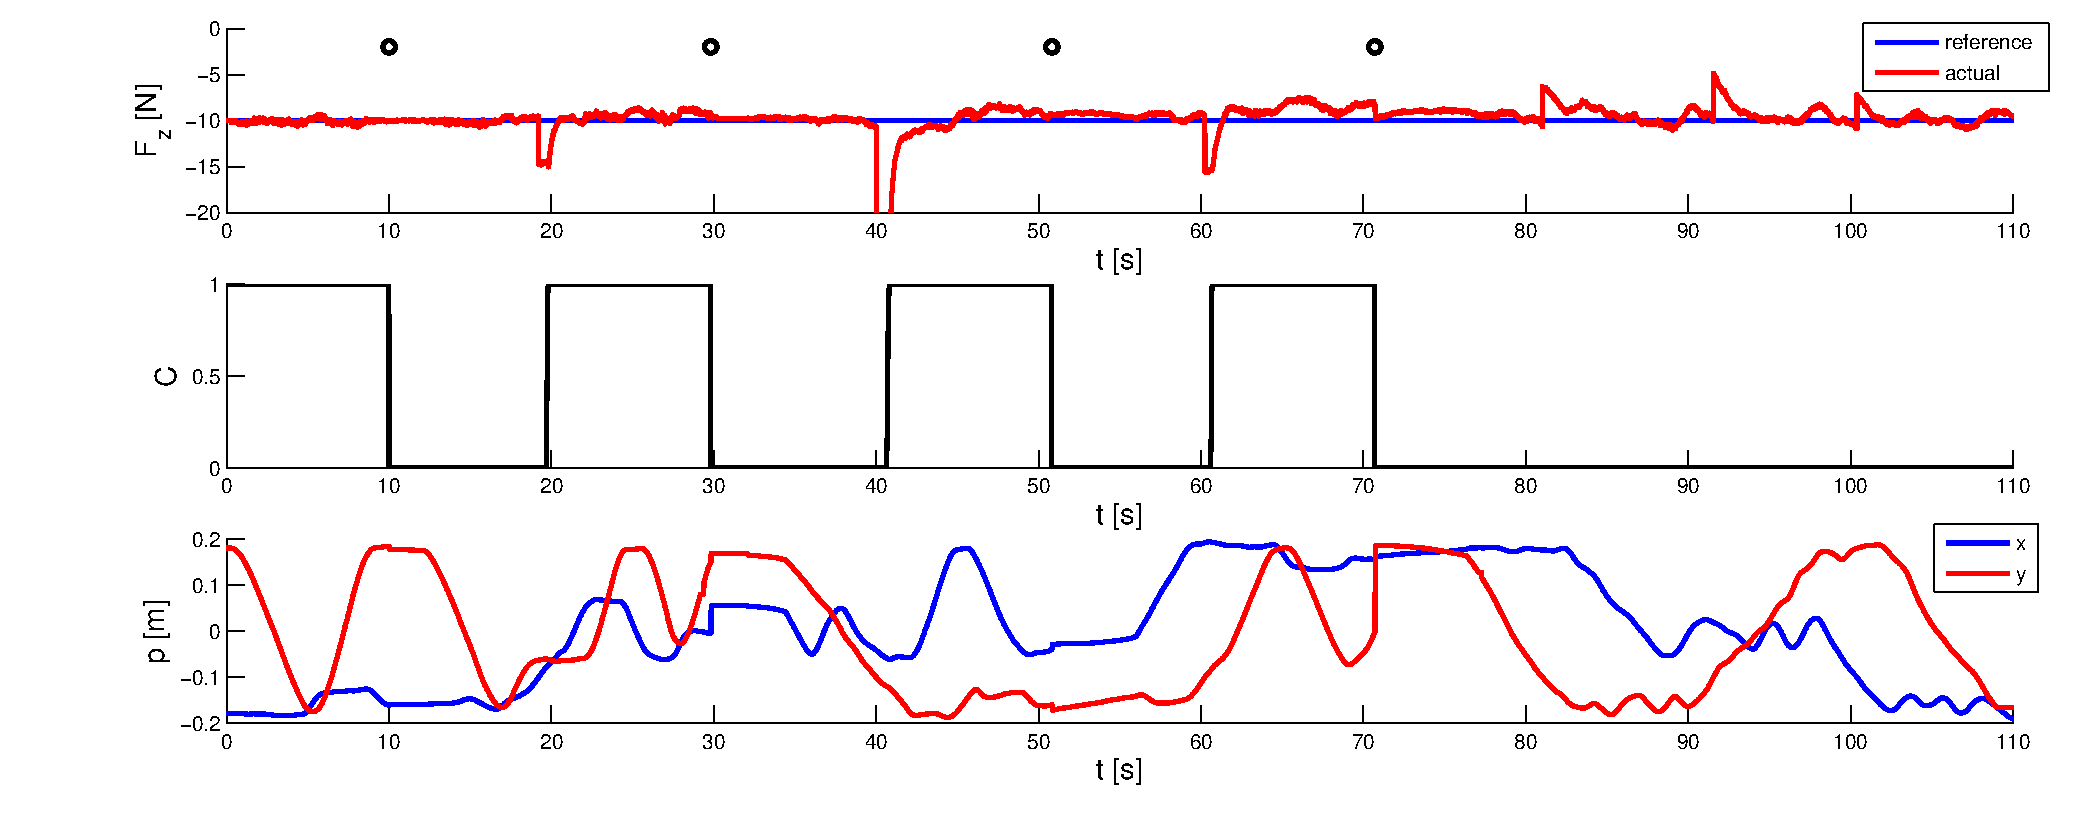
\includegraphics[width=0.85\textwidth]{Luka/results2.eps}
  \caption{Results of the experiments - task execution and shared control. The top graph shows the reference and actual force in z-axis. The middle graph shows the control responsibility factor $C$ (1 = demonstrator, 0 = robotic skill). The bottom graph shows the position of the manipulator in x-y plane. Training data updates are indicated by black dots on the top and correspond to the time stamps at the top of Fig. \ref{fig:models}.}
  \label{fig:force}
  \vspace{-4 mm}
\end{figure*}

The parameters for shared-control system were also set experimentally. The threshold of model's receptive field activation that determines whether the control is given to the demonstrator or robotic skill was set to $w_{th}=0.5$. We recommend following $w_{th}\leq w_{gen}$ in order not to create new models while the demonstrator does not have the control responsibility. The parameter related to smooth transition of control responsibility between the human and robotic skill was set to $d=0.05$. If slower transition phase is preferred then this parameter should be increased. Accumulation buffer length was set to $N_{acc}=1000$. This parameter should be lower if more frequent updates of robotic skill are preferred.

\section{Results}
The results of the robot learning during the experiment are shown in Fig. \ref{fig:models}. Each column represents the different stage of training data update. The time stamps of the update application are displayed on the top. The top row shows the acquired models (robotic skill) for manipulator's displacement of reference position from the actual position in z-axis. The middle row shows the force prediction error of the models at each stage. The bottom row shows the motion of the robot manipulator (thick black and green line) on the object's surface (thin black rectangle). The black line shows the trajectory when the demonstrator had the control over the robotic manipulator's force production task. The green line shows the trajectory when robotic skill had the control over the robotic manipulator's force production task. The red crosses show the centres while blue ellipses show the threshold activation ranges $w_{th}$ of the currently available local models that are part of robotic skill.

From the graphs we can see how the overall model was gradually updated when the demonstrator was teaching at various sections of the surface. In the first stage the local models are only created around the state region where the demonstration was initially performed. In the other sections of the surface the prediction error is naturally high due to non-existence of local models. When the demonstration progressed additional models were generated in the other sections. In the last training data update the local models fully covered the space of the given task and the robotic manipulator entered the fully autonomous stage (i.e. autonomously produced the desired force based on the position on the x-y plane).

Additional results are shown in Fig. \ref{fig:force}. The interaction force control as a result of adjusted commanded (reference) position along z-axis is shown in the top graph. We can see that the desired force was maintained relatively well by both the demonstrator and the obtained robotic skill. The black dots in the top show the time stamps when the training data was updated and correspond to the update times in Fig. \ref{fig:models}. The control responsibility factor $C$ is shown in the middle graph. The position of the manipulator in x and y-axis is shown in the bottom graph. Initially, $C$ was equal to one as there were no models present. After the prescribed amount of training data $N_{acc}$ was accumulated the robotic skill was updated with the learnt models in the demonstrated state region. Demonstrator then remained in that state region to examine the performance of the obtained robotic skill. Consequently $C$ became zero to give the control responsibility to the robotic skill. This procedure then repeated for the remaining three state regions of the task defined by different stiffness of the plane.

By observing the control responsibility we can see how it switched from demonstrator to the currently available local models. After each model update the control responsibility was shifted from the demonstrator to the robotic skill as the current position of robotic manipulator was within the predefined range of the existing models ($w_{max}>w_{th}$). The demonstrator could then move within the area where the teaching was already done to observe how the obtained robotic skill performs the task autonomously (see thick green lines in bottom graph of Fig. \ref{fig:models}). When the validation was done, the demonstrator moved to the unexplored area to perform the teaching there (see thick black lines in the bottom graph of Fig. \ref{fig:models}).


\section{Discussion}
The aim of this paper was to propose a new shared-control approach for human-in-the-loop robot teaching, and realise it for a non-trivial task as a proof-of-concept. In the hardware experiments conducted, the demonstrator could examine, online, the performance of the robotic skill being built during the demonstration stage, and gradually transform the robot to be an expert in the full allowed workspace. In the current implementation, we did not implement the ability of the demonstrator to remove already built local models. This was not needed in the current experiments as the demonstrator was expert and did not teach {\it bad} policies. This feature can be incorporated into the current system as a manual interface (e.g. pushing a button) or an automatic mechanism that detects the demonstrator's effort to correct a bad policy.

In future we will introduce an upgrade to the proposed framework where the human demonstrator will be able to remove the models, if the robotic skill performance is unsatisfactory after online examination. This will clear the undesired models in designated state region and allow corrections by re-teaching. Parameter $\lambda$ could be used in this case to forget the undesired models. In addition, we will experimentally explore the influence of system parameters on the performance of the proposed method.

By observing the obtained models in Fig. \ref{fig:models}, we can see that there is a considerable prediction error on the borders between two objects of different stiffness. This can be attributed to the difficulty of regression method to model larger discrete transitions within the training data output.

Potential disadvantage of the proposed method compared to \cite{Peternel2013b} and \cite{Zamani2015} is that the demonstrator has to manually inspect and determine the quality of the robotic skill. However, this gives the demonstrator more control over the learning. In addition, no extra cost functions are required to determine the quality automatically, as they can be hard to acquire and can produce unreliable results in complex tasks.